\subsection{Product perspective}
The product will be used by farmers, policy makers and agronomists.
\subsubsection{Scenarios}

\paragraph{Scenario 1: Farmer registration}\mbox{} \\

Ishaan receives an e-mail from administration that redirects him to the DREAM website registration page. He registers by providing his email address, name, surname, farm name and finally location which he provides by means of the geo-tracking functionality of his smartphone. The system checks that the email address isn't already registered, then sends a validation email to Ishaan.

After validation, the system fetchs Ishaan's district and mandal, based on his location. It then displays rainfall conditions and predictions, respectively based on Ishaan's mandal and location, on the homepage of Ishaan. It then fetchs the policy makers corresponding to this area. The system sends a notification to the policy maker in charge of the area to acknowledge the registration of Ishaan.

\paragraph{Scenario 2: Production data and type release}\mbox{} \\

Shyla has just finished his crop. She measures her production. She logs in on the DREAM platform where she had already registered. She goes to the page "Release production". She fills the following sections: seed variety, seed rate, production amount, surface area of the cultivated fields, amount of water consumed, start and end date.

\paragraph{Scenario 3: Discussion forum creation}\mbox{} \\

Dhruv's old tractor is broken. He wonders if he should try to repair it, if possible, and if not, what modern model he should choose. He looks for feedbacks on the forum discussion of the DREAM platform. As he can't find any on the kind of engine he owns, he creates a new topic, explains his issue and waits for answers.

\paragraph{Scenario 4: Prediction check}\mbox{} \\

Ashwin wants to know what are the soil and weather conditions of his mandal to correctly dose his fertilizer. He logs in on the DREAM platform. He goes to the homepage. He checks the soil moisture data, weather conditions and predictions.

\paragraph{Scenario 5: Request for production data and type release}\mbox{} \\

Between April and October, Amar crops and harvests rice during the so-called "Kharif"season. In November, he receives a notification from DREAM that urges him to release his production data - seed variety, seed rate, production amount, surface area of the cultivated fields, amount of water consumed, start and end date - by the end of the month. He instantly performs. On the first of December, a notification telling the completeness of the database gathering the production data of the farmers in Amar's area based on the location of his farm is sent by the system to the dedicated policy maker.

\paragraph{Scenario 6: Research among discussion forums}\mbox{} \\

Diya is not sure about the law regarding some specific fertilizer. She looks for discussion forums on DREAM. She uses as keywords "law", the name of the fertilizer and she filters the results to get late discussions - she knows that the law has changed in the previous years. She finds some farmer whose response handles her issue. Since she wants some more precision, she contacts the farmer, via DREAM, in a private discussion.

\paragraph{Scenario 7: Help request notification}\mbox{} \\

Sahil receives a notification from his policy maker suggesting him some practices fertilizer,crops and overall practices to improve his productivity and a proposal for a specific help request.

\paragraph{Scenario 8: Well performing farmers identification}\mbox{} \\

Nikhil is a policy maker. On December, 1st, he receives a notification from DREAM telling that all farmers of his area have delivered their production data. He selects some performance metrics among those proposed. The systems ranks the farmers accordingly and displays the ranking. Nikhil selects the farmer that he wants to congratulate. He sends to each one a message via DREAM, and ticks a box to send an e-voucher that the system generates and enclose. In the messages, Nikhil asks for best practices to the farmers.

\paragraph{Scenario 9: Poorly performing farmers identification}\mbox{} \\
% del line : Based on the data of these farmers and figures of the previous years, the system computes the personalized suggestions to each of them (should/could it be computed ?) ????
Ananya is a policy maker. On December, 1st, she receives a notification from DREAM telling that all farmers of her area have delivered their production data. She selects some performance metrics among those proposed. The systems ranks the farmers accordingly and displays the ranking. Ananya selects the farmers that may require help. She sends them a message via DREAM to tell them these suggestions and propose them to be helped.

\paragraph{Scenario 10: Major issues identification}\mbox{} \\

Nila is a policy maker. Crop is coming to end. She wants to correctly understand the issues that face the farmers of her area, in order to ask relevant questions to well performing farmers. She spends some time on forum discussions and note the most repeating concerns of farmers.

\paragraph{Scenario 11: Help request}\mbox{} \\

Tamia requires the insight of some expert on crops for the coming seeding. She goes to the "help request" section. She sends message. Based on her location, the system forwards the message to the adequate policy maker. The latter will send the request to an agronomist, who will afterwards contact Tamia.

\subsubsection{Product functions}

\begin{itemize}
	\item
	R1: The system should integrate a calendar that rythms the alternance of cropping season/release period/analysis period. 
	\item
	R2: Two weeks before the end of the release period, DREAM should recall the farmer to confirm the batch of production (if the farmer didn't confirm it yet).
	\item
	R3: Two weeks before the end of the analysis period, DREAM should recall the policy maker to identify well and poorly performing farmers (if not done).
	\item
	R4: Two weeks before the end of the analysis period, DREAM should recall the policy maker to send messages/incentives/help proposal to farmers, if some of the well or poorly performing ones weren't contacted yet.
	\item
	R5: DREAM should enable messaging between farmers and a farmer and a policy maker from the same area.
	\item
	R6: When an area is given, DREAM should fetch the policy maker in charge of it.
	\item
	R7: DREAM should enable any farmer to create a discussion forum, with a title, tags and filters.
	\item
	R8: When requested, DREAM should provide discussion forums ordered by semantic proximity of a given topic.
	\item
	R9: DREAM should enable unlimited answers in the thread of a forum.
	\item
	R10: When a location is asked and the user has agreed so, DREAM should fetch the position thanks to the GPS functionality of a device.
	\item
	R11: Given a date and a location, DREAM should fetch from the external databases the  closest and latest weather conditions.
	\item
	R12: Given a date, a location and a number of days, DREAM should fetch from the external databases the  closest and most adequate (with respect to the number of days of prediction) weather predictions.
	\item
	R13: Given a date and a location, DREAM should fetch from the external databases the  closest and latest soil moisture data (that is, figures and locations).
	\item
	R14: Given a date and a location, DREAM should fetch from the external databases the  closest and latest soil organic carbon data (that is, figures and locations).
	\item
	R15: Given a date and a location, DREAM should fetch from the external databases the  closest and latest vegetation index data (that is, figures and locations).
	\item
	R16: Given a list of figures and locations, DREAM should display them on an interactive map, with a nice legend.
	\item
	R17: On a move, the map displayed should be reactive. That is to say: it should query new values to fit in the new spatial frame.
	\item
	R18: DREAM should have a clock synchronous with the Indian time zone and Gregorian calendar.
	\item
	R19: Given a metric and a batch from a location, DREAM should fetch the required data at the date that correspond to the batch. The system should then correctly compute the performance.
	\item
	R20: The system should be able to rank a list of farmers during a given season with respect to a metric.
	\item
	R21: Given a two dates and a farmer identity, DREAM should fetch from the water irrigation system the total amount of water consumed during the time-lapse by the farmer.
	\item
	R22: If any necessary piece of information is missing at some point of a process, DREAMS should display an error message.
	\item
	R23: Given a user identity, DREAMS should be able to access all the personal data of this user.
	\item
	R24: When a policy maker decides to make an incentive, DREAMS should create via an external API an e-voucher of the amount wanted. 
	\item
	R25: Given a farmer identity, DREAM should be capable of fetching the corresponding batch.

\end{itemize}

\subsubsection{Assumptions, dependencies and constraints}
%TODO
\begin{itemize}
	\item
	A1: Cropping seasons are the same on the whole Telengana State and follow the Kharif/Rabi calendar, see Figure \ref{fig:seasons}, as related in \cite{seasons}.
	\item
	A2: Farmers put rightful information on their location and data on their production. Fraud is possible but it is the responsibility of policy makers to prevent it, with the help of agronomists.
	\item
	A3: If a policy maker is missing at some farmer's registration, he/she will be found before the end of the cropping season.
	\item
	A4: All users that register have access to internet in some way and have access to the application.
	\item
	A5: All humidity data are collected through the database of the NICES project. The system thus doesn't require its own sensors.
	\item
	A6: To avoid money transfers and check the use of the money, incentives are sent as e-vouchers. This decisions was supported by the stakeholder, see \cite{git}.
	\item
	A7: The irrigation system is supposed to provide the water consumption data thanks to an external API. 
	
\end{itemize}

\begin{figure}[H]
	
	\centering
	
	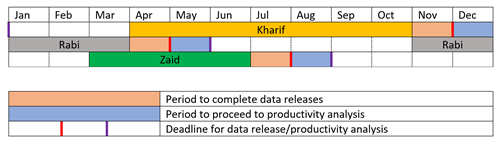
\includegraphics[width=\columnwidth]{Images/croping-seasons-calendar.png}
	
	\caption{Seasons}
	
	\label{fig:seasons}
	
\end{figure}


\subsubsection{Mapping on goals}
\begin{table}[H]
	\centering
	\begin{tabularx}{\linewidth}{|l|X|X|}
		\hline
		\multicolumn{1}{c|}{\textit{\textbf{Goals}}} & \multicolumn{1}{c|}{\textit{\textbf{Assumptions}}} &
		\multicolumn{1}{c|}{\textit{\textbf{Requirements}}}
		                                                 \tabularnewline \hline
		G1.1.1 &
		A1,A3,A4&
		R1,R2,R3,R4,R5,R6,R25
		\tabularnewline
		\hline
		G1.1.2 & 
		A3,A4&
		R5, R23
		\tabularnewline
		\hline
		G1.2.1 & 
		A4&
		R7
		\tabularnewline
		\hline
		G1.2.2 & 
		A4&
		R8,R18
		\tabularnewline
		\hline
		G1.2.3 & 
		A4&
		R9,R18
		\tabularnewline
		\hline
		G1.2.4 & 
		A4&
		R5,R23
		\tabularnewline
		\hline
		G2.1 & 
		A4&
		R9,R10,R11,R12,R16,R17,R18
		\tabularnewline
		\hline
		G2.2 & 
		A4,A5&
		R9,R10,R11,R13,R16,R17,R18
		\tabularnewline
		\hline
		G2.3 & 
		A4&
		R9,R10,R11,R14,R16,R17,R18
		\tabularnewline
		\hline
		G2.4 & 
		A4&
		R9,R10,R11,R15,R16,R17,R18
		\tabularnewline
		\hline
		G3.1 & 
		A2,A4,A7&
		R9,R10,R11,R12,R13,R14,R15,R16,R17,R18,R19,R20,R21
		\tabularnewline
		\hline
		G3.2 & 
		A4,A6&
		R5,R24
		\tabularnewline
		\hline
		G3.3 & 
		A4&
		R5
		\tabularnewline
		\hline
		G3.4 & 
		A4&
		R5
		\tabularnewline
		\hline
	\end{tabularx}   
\end{table}


